\documentclass[12pt]{iopart}
\newcommand{\gguide}{{\it Preparing graphics for IOP Publishing journals}}
%Uncomment next line if AMS fonts required
%\usepackage{iopams}  
\usepackage[dvipdfmx]{graphicx}
\usepackage{afterpage}
\usepackage{braket}
\usepackage{comment}
\newcommand{\average}[1]{\ensuremath{\langle#1\rangle} }

\begin{document}
\title{Heat transport via a local two-state system}
\author{Masanari Kato$^1$, Takeo Kato$^1$ and Keiji Saito}
\address{$^1$ IOP Publishing, Temple Circus, Temple Way, Bristol BS1 6HG, UK}
\ead{kato@issp.u-tokyo.ac.jp}
\vspace{10pt}
\begin{indented}
\item[]February 2014
\end{indented}

\begin{abstract}
test
\end{abstract}

\section{Introduction}
\section{Model and Exact Formula}
In this section, we explain the model which describes the heat transport via a local two-state system.
Then, we derive the exact formula of liner heat conductance in this system by using the Keldysh formalism.

When we discuss the heat transport via a zero-dimensional object, we should consider the system where a local oscillator is localized between two phonon baths. 
Now, we adopt the double well potential as the local oscillator because this potential can denote the boson interaction caused by nonlinearity. In reality, this system can be implemented as the molecular junction or the Josephson junction in the super conducting circuit\cite{experiment?}(Fig. \ref{fig:j_c}).
\begin{figure}[tb]
	\centering
	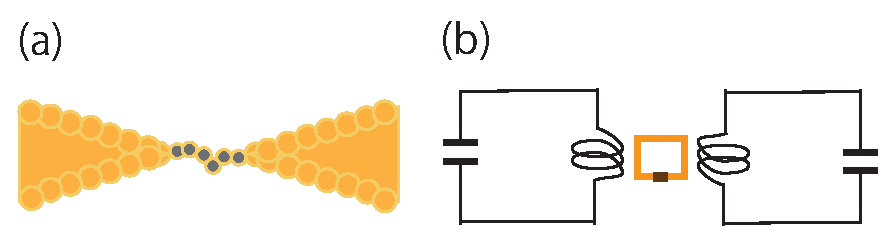
\includegraphics[width=130mm]{j_c.eps}
	\caption{(a)molecular junction, (b)Josephson junction in the super conducting circuit}
	\label{fig:j_c}
\end{figure}
At low temperature, when the potential barrier is infinitely higher than the energy level difference from the ground state to the first excited state, the local oscillator can be regarded as the two-state system described by the ground state where the system is localized at the right or left well.
Then, we can relate the two-state system to the pseudo-spin system. 
Then, the Hamiltonian of local oscillator is described by  the Pauli matrix $\sigma_{i}(i:x,y,z)$ as
\begin{eqnarray}
	H=\frac{\hbar \Delta}{2} \sigma_x+\frac{\hbar\epsilon}{2}\sigma_z,
\end{eqnarray}
where $\Delta$ is the tunneling amplitude and $\epsilon$ is the bias of the system, i.e., the difference in the ground-state energies of the local two states.
In this study, we assume the symmetric double well, i.e., $\epsilon=0$.
Then, the local two-state system coupling to two phononic baths is described by the spin-boson Hamiltonian:
\begin{eqnarray}
	H=\frac{\hbar \Delta}{2} \sigma_x 
	+\sum_{\nu=L,R}\sum_{\nu k}\hbar \omega_{\nu k } b_{\nu k}^{\dagger} b_{\nu k}
	+ \frac{\sigma_z}{2} \sum_{\nu=L,R}\sum_{\nu k} \hbar \lambda_{\nu k}(b_{\nu k}+b_{\nu k}^{\dagger}),
	\label{Hamiltonian}
\end{eqnarray}
where $\omega_{\nu k}$, $b_{\nu k}$ is the frequency and annihilation operator of phonon with the wavenumber $k$ in the $\nu$th bath, and $\lambda_{\nu k}$ is the coupling strength between the local two-state system and phonons in two phononic baths.
(Fig. \ref{fig:system_image}) is the image? of this system.
\begin{figure}[tb]
	\centering
	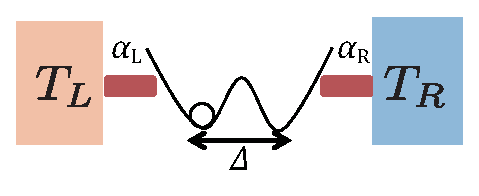
\includegraphics[width=100mm]{system_image.eps}
	\caption{The two-state system coupling to two phononic baths. If the temperature of two baths is slightly different, phonon can be transported from one bath to another.}
	\label{fig:system_image}
\end{figure}
The spectral function defined as  
\begin{eqnarray}
	I_{\nu}(\omega)&\equiv&\sum_{\nu k} \lambda_{\nu k}^2\delta(\omega-\omega_{\nu k})
\end{eqnarray}
characterizes the behavior of heat transport under the spin-boson model.
We assume that the spectral function takes the form of power law:
\begin{eqnarray}
	I_{\nu}(\omega)&=&\alpha_\nu \tilde{I}_\nu (\omega), \label{spect} \\
	\tilde{I}_\nu(\omega)&=&2\omega_c^{1-s}\omega^s f(\omega/\omega_c),
\end{eqnarray}
where $\alpha_{\nu}$ is the dimensionless coupling strength between the local two-state system and the $\nu$th heat bath, $\omega_c$ is the cutoff frequency satisfying $\omega_c\gg\Delta,\epsilon$, and $f(\omega/\omega_c)$ is the cutoff function in the range [0,1]. For simplicity, we assume the cutoff function $f(\omega/\omega_c)$ takes the form of step function $\theta(\omega_c-\omega)$.
The case of $s=1$ is called ``ohmic'' and the ohmic case is studied in detail as we discussed in the section 1. 
The case of $s>1$ and $ s<1$ is called ``super-ohmic" and ``sub-ohmic", respectively, 
and these non-ohmic case is our main interest.
Starting with this setup, we derive the exact formula of thermal conductance under the spin-boson model by using Keldysh formalism.
 
First, we define the operator of the heat current flowing from the $\nu$th bath into the local two-state system as 
\begin{eqnarray}
	J_\nu\equiv\frac{dH_{\mathrm{bath},\nu}}{dt},
	\label{current_opperator}
\end{eqnarray}
where the Hamiltonian of the $\nu$th bath is defined as $H_{\mathrm{bath},\nu} \equiv\sum_k\hbar \omega_{\nu k } b_{\nu k}^{\dagger} b_{\nu k}$.
This operator follows the Heisenberg's equation of motion, then 
\begin{eqnarray}
	J_\nu&=&-\frac{i}{\hbar}[H_{\mathrm{bath},\nu},H]\\
	&=&-i \sum_k\frac{\lambda_{\nu k}}{2}\hbar\omega_{\nu k}\sigma_z(-b_{\nu k}+b_{\nu k}^{\dagger}).
\end{eqnarray}
The ensemble average of heat current $\average{J_\nu(t)}=\mathrm{Tr}[\rho J_\nu(t)]$, where $\rho$ is the density matrix of initial state, is calculated as 
\begin{eqnarray}
	\average{J_\nu(t)}=\mathrm{Re}\left . \left[\sum_k\frac{\hbar^2\omega_{\nu k} \lambda_{\nu k}}{2}
	G^{<}_{\sigma_z,b_{\nu k}^{\dagger}}(t_1,t_2)\right] \right |_{t_1=t_2=t},
\end{eqnarray}
where the lesser Green's function is defined as 
\begin{eqnarray}
	G^{<}_{\sigma_z,b_{\nu k}^{\dagger}}(t_1,t_2)\equiv-\frac{i}{\hbar}\average{b_{\nu k}^{\dagger}(t_2)\sigma_z(t_1)}.
\end{eqnarray}
Then, by using Keldysh formalism, we can derive the heat current at the steady state\cite{Saito08}:
\begin{eqnarray}
	\average{J_\nu}=\frac{\hbar}{4}\int_{0}^{\infty}d\omega\, 
		\hbar \omega\left[ 
			\mathrm{Im}[G_{\sigma_z,\sigma_z}^{r}(\omega)]I_\nu(\omega)n_\nu( \hbar\omega)-
			iG^{<}_{\sigma_z,\sigma_z}(\omega)\frac{I_\nu(\omega)}{2}
		\right],
\end{eqnarray}
where  $n_\nu( \hbar\omega)$ means the Bose-Einstein distribution function and the retarded Green's function is defined as 
\begin{eqnarray}
	G_{A,B}^r(t_1,t_2)\equiv -\frac{i}{\hbar}\theta(t_1-t_2)\average{[A(t_1),B(t_2)]}.
\end{eqnarray}
Here, we introduce the quantity $\gamma_\nu$ which denotes the symmetry of coupling to the two baths:
\begin{eqnarray}
	\gamma_\nu=\frac{\int_0^{\infty}d\omega\,\hbar\omega G_{\sigma_z,\sigma_z}^{<}(\omega)I_\nu(\omega)}	{\sum_{\nu'=L,R}\int_{0}^{\infty}d\omega\,\hbar\omega G_{\sigma_z,\sigma_z}^<(\omega)I_{\nu'}(\omega)}.
\end{eqnarray}
Remarking the conservation law of the particle number $\average{J _L}+\average{J_R}=0$, $\average{J_L}$ can be denoted as follows by $\gamma_{\nu}$
\begin{eqnarray}
	\average{J _L}&=&\gamma_R\average{J_L}-\gamma_L\average{J_R}\\
	&=&\frac{1}{4}\int_0^{\infty}d(\hbar\omega)\,
	\hbar\omega\mathrm{Im}[G^r_{\sigma_z,\sigma_z}(\omega)]
	\left[\gamma_RI_L(\omega)n_L(\hbar\omega)-\gamma_LI_R(\omega)n_R(\hbar\omega)\right].
\end{eqnarray}
Here, we assume $\tilde{I}_L(\omega)=\tilde{I}_R(\omega)=\tilde{I}(\omega)$, then $\average{J_L}$ is
\begin{eqnarray}
	\average{J _L}=\frac{\alpha_L\alpha_R}{4(\alpha_L+\alpha_R)}\int_0^{\infty}d(\hbar\omega)
		\hbar\omega\mathrm{Im}[G^r_{\sigma_z,\sigma_z}(\omega)]
		\tilde{I }(\omega)\left[n_L(\hbar\omega)-n_R(\hbar\omega)\right].
		\label{exact_current}
\end{eqnarray}
In the linear response regime, thermal conductance is defined as
\begin{eqnarray}
	\kappa\equiv \lim_{\Delta T \rightarrow 0} \frac{\average{J_L}}{\Delta T}.
	\label{den_kappa}
\end{eqnarray}
Finally, we can get the exact formula of thermal conductance: 
\begin{eqnarray}
	\kappa=\frac{k_B\alpha\omega_c^{1-s}}{4}\int_{0}^{\infty}d(\hbar\omega)\mathrm{Im}
	[\chi(\omega)]\omega^s\left[\frac{\beta\hbar\omega/2}{\mathrm{sinh}(\beta\hbar\omega/2)}\right]^2,
	\label{exact_kappa}
\end{eqnarray}
where we assumed  the symmetric coupling strength $\alpha=\alpha_L=\alpha_R$ and substituted the response function $\chi(\omega)$ for $G^r_{\sigma_z,\sigma_z}(\omega)$ by considering the linear response theory.
Eq. (\ref{exact_kappa}) is the main result in this section.
When we evaluate the value of conductance (\ref{exact_kappa}), we have to calculate the response function $\mathrm{Im}[{\chi}(\omega)]$. But, except the special case like ``Toulouse limit'' ($\alpha=1/2$ in the ohmic case), it is difficult to analytically calculate $\mathrm{Im}[{\chi}(\omega)]$.
Here, in this study, we numerically evaluate $\mathrm{Im}[{\chi}(\omega)]$ by the Monte Carlo method.
Although we explain how to numerically calculate $\mathrm{Im}[{\chi}(\omega)]$ in section 4 in detail,
in the next section, we derive the approximate formulas of thermal conductance (\ref{exact_kappa}) in three different situations.  
\section{Approximate Formulas}
%==========================================================
\subsection{sequential tunneling}
consider $T\simeq\mathit{\Delta}_{\mathrm{eff}}$\\
then the spectral function 
\begin{eqnarray}
	S(\omega)\equiv\frac{\mathrm{Im}[\chi(\omega)]}{\omega }
\end{eqnarray}
\begin{eqnarray}
	S(\omega) = \frac{\Delta}{\pi} \left[\delta(\omega-\Delta)+\delta(\omega+\Delta) \right]
\end{eqnarray}
is approximated as 
\begin{eqnarray}
	S(\omega)\simeq A\delta(\omega-\mathit{\Delta}_{\mathrm{eff}})+\delta(\omega+\mathit{\Delta}_{\mathrm{eff}})
\end{eqnarray}
where $\delta(x)$ is delta function.
then we apply  Kramers-Kronig relation
\begin{eqnarray}
	\frac{1}{\pi}\int_{-\infty}^{\infty}d\omega S(\omega)&=&\frac{1}{\pi}\int_{-\infty}^{\infty}d\omega \frac{\mathrm{Im}[\chi(\omega)]}{\omega}\\
&=&\mathrm{Re}[\chi (0)]
\end{eqnarray}
\begin{eqnarray}
	\chi_m \equiv \lim_{\epsilon \rightarrow 0} \frac{\langle \sigma_z \rangle}{\epsilon}
\end{eqnarray}
in the super ohmic and ohmic case $\chi_m=2\mathrm{tanh}(\beta \mathit{\Delta}_{\mathrm{eff}}/2)/\mathit{\Delta}_{\mathrm{eff}}$.
then  (\ref{exact_kappa}) is 
\begin{eqnarray}
	\kappa\simeq \frac{\pi\alpha\omega_c^{1-s}}{4}\frac{ \Delta_{\mathrm{eff}}^{s}}{2n(\Delta_{\mathrm{eff}})+1}\left[\frac{\beta\Delta_{\mathrm{eff}}/2}{\mathrm{sinh}{(\beta\Delta_{\mathrm{eff}}/2})}\right]^{2}
\end{eqnarray}
%==========================================================
\subsection{cotunneling}
consider lowtemperature $T\ll\mathit{\Delta}_{\mathrm{eff}}$, where $\mathit{\Delta}_{\mathrm{eff}}$is  abatically renormalized tunnneling rate.\\
generalized Shiba's relation
\begin{eqnarray}
	 \lim_{\omega \to 0+} \frac{\mathrm{Im}[\chi(\omega)]}{\omega^{s}}=2\pi\alpha\left(\frac{\chi_m}{2}\right)^{2}
\end{eqnarray}
where $\chi_m$ is susceptibility\\
then (\ref{exact_kappa}) is 
\begin{eqnarray}
	\kappa&\simeq& \frac{\pi\omega_c^{s-1}\chi_m^2}{8}\int_{0}^{\omega_{c}}d\omega  I_L(\omega)I_R (\omega)\left[\frac{\beta\omega/2}{\sinh{(\beta\omega/2)}}\right]^{2}
\end{eqnarray}
\begin{eqnarray}
	\kappa\simeq \frac{\pi\omega_c^{1-s}}{8}\left( \alpha \chi_m \right)^2 F(s)T^{2s+1}
	\label{cond_lowtemp},\\
	F (s)=\int_{0}^{\beta\omega_{c}}dx  x^{2s}\left[\frac{x/2}{\sinh({x/2})}\right]^{2}
\end{eqnarray}
%==========================================================
\subsection{incoherent  tunneling}
consider $T \gg \Gamma$. master eq.
\begin{eqnarray}
	\frac{dP_+(t)}{dt}=\Gamma P_-(t) - \Gamma P_+(t)
\end{eqnarray}
Fermi's golden rule
\begin{eqnarray}
	\Gamma&=&\left({\frac{\Delta}{2}}\right)^2\int_{-\infty}^{\infty}dt \ e^{-Q(t)},\label{Gamma} \\
		Q(t)&=&\int_{0}^{\infty}d\omega \frac{I(\omega)}{\omega^2}\left \{ \mathrm{coth\left(\frac{\beta \omega}{2}\right)[1-\mathrm{cos}(\omega t)]+\it{i} \ \mathrm{ sin}(\omega t)}\right \}
\end{eqnarray}
\begin{eqnarray}
	\langle\sigma_z(t)\rangle=\frac{P_+-P_-}{P_++P_-} =e^{-2\Gamma t}
	\label{sigma_z}
\end{eqnarray}
\begin{eqnarray}
	C(t)=\langle \sigma_z(t) \sigma_z(0) \rangle=e^{-2\Gamma|t|}  
\end{eqnarray}
\begin{eqnarray}
	C(t)&\equiv&\langle\sigma_z(t)\sigma_z(0)+\sigma_z(0)\sigma_z(t)\rangle/2\\
		&=&\langle \sigma_z(t) \sigma_z(0) \rangle\\
		&=&e^{-2\Gamma|t|}
\end{eqnarray}
Fourier transformation
\begin{eqnarray}
	C(\omega)=\frac{4\Gamma}{\omega^2+4 \Gamma^2}
\end{eqnarray}
fluctuation-dissipation theorem
\begin{eqnarray}
	 C(\omega)=\mathrm{coth}\left(\frac{\beta\omega}{2}\right)\mathrm{Im}[\chi(\omega)]
\end{eqnarray}
$T\gg\Delta$
\begin{eqnarray}
	C(\omega)&\simeq& 2\frac{\mathrm{Im}[\chi(\omega)]}{\beta \omega}=2TS(\omega)
\end{eqnarray}
then the spectral function is
\begin{eqnarray}
	S(\omega)=\frac{2\Gamma/T}{\omega^2+4\Gamma^2}\simeq \frac{2\Gamma}{\omega^2T}
\end{eqnarray}
then (\ref{exact_kappa}) is 
\begin{eqnarray}
	\kappa&\simeq&\frac{\alpha\omega_c^{1-s}}{4}\int_{0}^{\omega_c}d\omega \frac{2\Gamma}{T}\omega^{s-1}\left[\frac{\beta\omega/2}{\sinh{(\beta\omega/2)}}\right]^{2}\\
	&=&\frac{\alpha\omega_c^{1-s}}{2}G(s)\Gamma T^{s-1}	
\end{eqnarray}
\begin{eqnarray}
	G(s)=\int_{0}^{\beta \omega_c}dx\, x^{s-1}\left[\frac{x/2}{\sinh{(x/2)}}\right]^{2}
\end{eqnarray}
ohmic case
\begin{eqnarray}
	\kappa\simeq\frac{\sqrt{\pi}\Gamma(\alpha)}{4\Gamma(\alpha+1/2)}\frac{\Delta^2}{\omega_c}	\left(\frac{\pi T}{\omega_c}\right)^{2\alpha-1}
\end{eqnarray}
sub ohmic case
\begin{eqnarray}
	\kappa\simeq\frac{\alpha\omega_c^{1-s}}{2}G(s)\frac{\Delta^2}{4}e^{-\frac{\beta \Lambda_1}{4}}\sqrt{\frac{\pi \beta}{\Lambda_2}}T^{s-1} 
\end{eqnarray}
where
\begin{eqnarray}
	\Gamma&=&\frac{\Delta^2}{4}e^{-\frac{\beta \Lambda_1}{4}}\sqrt{\frac{\pi \beta}{\Lambda_2}},\\
	 \Lambda_1&=&8T\alpha\Gamma(s-1)+16T\alpha\Gamma(s-1)\left(\frac{T}{\omega_c}\right)^{s-1}(2-2^{s-1})\zeta(s-1),\\
	 \Lambda_2 &=&T\left(\frac{T}{\omega_c}\right)^{s-1}2\alpha(2^{s+1}-1)\Gamma(s+1)\zeta(s+1)
 \end{eqnarray}
\begin{figure}[tb]
 \centering
 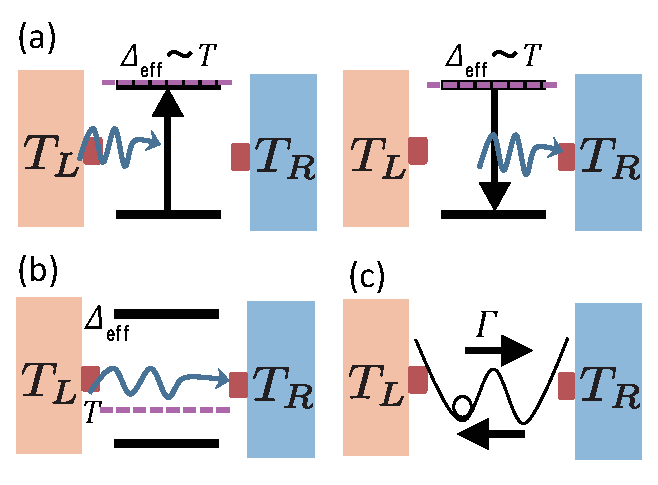
\includegraphics[width=100mm]{mechanism.eps}
 \caption{mechanism}
\end{figure}
\section{Monte Carlo method}
In this section, we map the spin-boson model to the Ising model with long-range interactions on the imaginary axis by deriving the partition function of the spin-boson model in the imaginary time form.
And, we explain how to numerically calculate the response function $\mathrm{Im}[\chi(\omega)]$ by Monte Carlo method to the long-range Ising model.

First, we divide the spin-boson hamiltonian (\ref{hamiltonian}) into two parts:
\begin{eqnarray}
	H&=&\frac{\Delta\sigma_x}{2}+H_z,\\
	H_z&=&\sum_{\nu=L,R}\sum_k\omega_{\nu k } b_{\nu k}^{\dagger} b_{\nu k}+\sum_{\nu=L,R}\sum_k \frac{\sigma_z}{2}\lambda_{\nu k}(b_{\nu k}+b_{\nu k}^{\dagger}).
\end{eqnarray}
Then, the partition function $Z=\mathrm{Tr}[e^{-\beta H}]$ can be described as
 \begin{eqnarray}
	Z&=&Z_++Z_-,\\
	Z_{\pm}&=&\bra{\pm}\mathrm{Tr_{\mathrm{boson}}}[e^{-\beta H}]\ket{\pm},
\end{eqnarray}
where $\ket{\pm}$ means the eigen state of $\sigma_z$, i.e., $\sigma_z\ket{\pm}=\pm1\ket{\pm}$, 
and  $\mathrm{Tr_{\mathrm{boson}}}$ means the trace for the boson's degree of freedom.
Here, we introduce $\tilde{\sigma}_x(u)$ defined as  
$
\tilde{\sigma}_x(u)\equiv e^{iH_zu}\sigma_xe^{-iH_zu},
$
then we can expand $Z_+$ into
\begin{eqnarray}
	Z_+&=&\mathrm{Tr_{\mathrm{boson}}}\left[\bra{+}e^{-\beta H_z}e^{-\int_{0}^{\beta}du \Delta \tilde{\sigma}_{x}(u)/2}\ket{+}\right]\\
	&=&\sum_{n=0}^{\infty}\mathrm{Tr_{\mathrm{boson}}}
	\left[\bra{+}e^{-\beta H_z }\int_{0}^{\beta}d\tau_1 \ldots \int_{0}^{\tau_{2n-1}-\tau_c} d\tau_{2n}
	\left(\frac{\Delta}{2}\right)^{2n}\tilde{\sigma}_x(\tau_1) \ldots \tilde{\sigma}_x(\tau_{2n})\ket{+}\right].
\end{eqnarray}
where $\tau_c$ is the cutoff on the imaginary time axis and it is given by $\tau_c=1/\omega_c$.
By calculating the trace for the boson's degree of freedom, we can derive the instanton-like partition function with n-kink pairs? \cite{Leggett87,Volker98}:
\begin{eqnarray}
	Z_+&=&Z_0\sum_{n=0}^{\infty}\left(\frac{\Delta\tau_c}{2}\right)^{2n}\int_{0}^{\beta}\frac{d\tau_1}{\tau_c} \ldots \int_{0}^{\tau_{2n-1}-\tau_c} \frac{d\tau_{2n}}{\tau_c}
	\mathrm{exp}\left[\sum_{j>i}^{2n}(-1)^{i+j}W(\tau_j-\tau_i)\right],
	\label{z_+}
\end{eqnarray}
where $Z _0$ is the partition function of  bosons in the heat bath,
and  $W(\tau)$ is given by 
\begin{eqnarray}
	W(\tau)&=&\int_{0}^{\infty}d\omega \frac{I(\omega)}{\omega^2}
	\frac{\mathrm{cosh}(\beta\omega/2)-\mathrm{cosh}(\beta\omega/2-\tau)}{\mathrm{sinh}(\beta\omega/2)}.
	\label{kink_interaction}
\end{eqnarray}
%付録?
We can calculate  $Z_{-}$ in the same way.
%
If we regard $\tilde{\sigma}_x(\tau_{j})$ as a kink charge, 
Eq. ($\ref{z_+}$) can be regarded as the ``kink'' representation of the one-dimensional Ising model with the  system states distinguished by the kink-degree of freedom $\{ \tilde{\sigma}_x(\tau_i)\}$.
Now, we consider rewriting it to the ``spin'' representation.
Generally, the partition function of  the one-dimensional Ising model with long-range interactions with the lattice constant $a$ 
is written in the kink representation as 
\begin{eqnarray}
	Z_{\mathrm{ising}}&=&\sum_{n=0}^{\infty}y^{2n}\int_{0}^{\beta}\frac{d\tau_1}{a} \ldots \int_{0}^{\tau_{2n-1}-a} \frac{d\tau_{2n}}{a}
	\mathrm{exp}\left[\sum_{j>i}^{2n}(-1)^{i+j}4U\left(\frac{\tau_j-\tau_i}{a}\right)\right],
	\label{Z_ising_kink}
\end{eqnarray}
where $U(\tau)$ is the kink-kink interaction, and $y$ is the chemical potential which satisfies $y=e^{2U(0)}$.
According to \cite{Volker98,Cardy81}, we can calculate the spin-spin interaction $V(n)$ from the kink-kink interaction $U(n)$ by the following recurrence relation:
\begin{eqnarray}
	V(n)=U(n+1)-2U(n)+U(n-1),\ (n:\mathrm{integer}>0),
	\label{V}
\end{eqnarray}
then, Eq. (\ref{Z_ising_kink}) is described by $V(n)$ as 
\begin{eqnarray}
	Z_{\mathrm{ising}}=\sum_{S_1 \ldots S_N}\mathrm{exp}\left[-\sum_{j>i}V(j-i)S_iS_j\right],
	\label{Z_ising_spin}
\end{eqnarray}
where $S_i,(i:\mathrm{integer})$ is the spin of the $i$th site, $N$ is the total number of sites, and $S_{i}$
satisfies the boundary condition $S_{i}=S_{i+N}$ (Fig. \ref{fig:ising_model}).
\begin{figure}[tb]
	\centering
	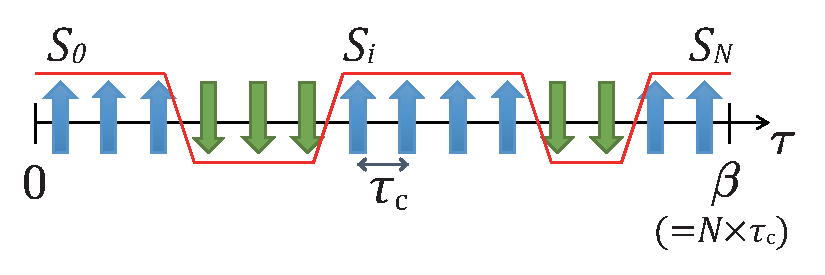
\includegraphics[height=4.0cm]{ising_model.eps}
	\caption{
	 the one-dimensional Ising model with long-range interactions on the imaginary $\tau$-axis.
	}
	\label{fig:ising_model}
\end{figure}
In this study, we divide $\beta$ in length on the $\tau$-axis into $N$ parts,
i.e., $\tau_c=\beta/N$.
Then, we put Ising spins on the each sites and chose $V(n)$ as Eq. (\ref{Z_ising_kink}) becomes our desiring partition function(\ref{z_+}).
Specifically, we decide $U(n)$ from $W(\tau)$, and calculate $V(n)$ by Eq. (\ref{V}).
Actually, we can derive $V(n)\propto n^{-(s+1)}$ for the large enough total number of sites $N$, i.e., $n/N\ll1$. 
In this way, we can map the spin-boson model to  the one-dimensional Ising model with long-range interactions.

Now, we remark the algebraic relation between the response function $\chi( \omega)$ and the spin-correlation function $C(\tau)$:
\begin{eqnarray}
	\chi(\omega)&=C(i\omega_n\rightarrow\omega+i\delta),\\
	\label{pade}
	C(i\omega_n)&=\int_{0}^{\beta}d\tau e^{i\omega_n \tau}C(\tau),\\
	\label{fourier}
	C(\tau)&=\average{\sigma_z(\tau)\sigma_z(0)},
\end{eqnarray}
where Eq. (\ref{pade}) means the analytic continuation.
These relations means we can derive $\mathrm{Im}[\chi( \omega)]$ by calculating $C(\tau)$.
And, we can derive $C(\tau)$ by calculating the spin correlation $\average{S_i S_0}$ of the long-range Ising model because they satisfies
$
\average{\sigma_z(\tau_i)\sigma_z(0)}\simeq \average{S_i S_0}.
$
%
In this study, we use the Monte Carlo method to calculate $C(\tau)$ of the Ising model derived from Eq. (\ref{Z_ising_spin}). But, it takes very long time to numerically calculate $C(\tau)$ because the Ising model derived from Eq. (\ref{Z_ising_spin}) has $r^{-(s+1)}$ long-range interactions. Especially, this problem notably appears in the low temperature. It is known that if you use the single flip method \cite{MetropolisMethod}, the relaxation time of the system diverges near the critical temperature (called ``critical slowing down''). 
This problem can be solved by the cluster-flip method like the Wolff algorithm\cite{Wolff89}.
In this study, we use an efficient Monte Carlo method based on the Wolff algorithm developed by E.Luijten \cite{Luijten95}.
The Luijten's algorithm utilizes the cumulative frequency distribution and in this algorithm we need not look at all spins in order to build a cluster but calculate the site at which the spin to add into a cluster first appears. 
Actually, we can realize more efficient implementation by making use of the bisection method to calculate the site.
In this way, we adopt the Wolff method utilizing the cumulative frequency distribution to calculate the spin correlation $\average{S_i S_0}$.


\section{Numerical result}

本章では、量子モンテカルロ法による数値計算の結果を示す。
まず、第\ref{sec:conductance}節において、一般の散逸における熱コンダクタンスの温度依存性を示し、どのようなトンネル過程が支配的となるかを近似解と比較することで具体的に調べる。
その後、第\ref{sec:phasetransition}節で、断熱くりこみの理論から示唆されるサブオーミック散逸における局在転移に関する計算結果を示す。
本章では$\omega_c=1$とし、すべてのエネルギースケールおよび温度スケールを$\omega_c$を単位として記述する。
%==================================================
\subsection{Thermal conductance}
\label{sec:conductance}

\subsubsection{Ohmic case}

オーミック散逸($s=1$)の熱コンダクタンスの温度依存性はすでに先行研究\cite{SaitoKato13}によって得られている(図\ref{fig:ohmic_result}参照)。オーミック散逸では$\Delta/\omega_c \ll 1$であれば、近藤模型と同様にエネルギーを$\Delta_{\rm eff}$でスケールすることによって、熱コンダクタンスが1つのユニバーサルな温度依存性を示すことが知られている。具体的には温度を$\Delta_{\rm eff}$によって規格化し、熱コンダクタンスを次元解析から$\Delta_{\rm eff}$で割って規格化すると、同一の曲線に乗ることがわかる(図\ref{fig:ohmic_result}参照)。

簡単にオーミック散逸におけるトンネル機構をまとめる。まず、散逸強度が$0<\alpha<1$の範囲にあるときは、低温において$T^3$に比例する熱コンダクタンスが得られる。これはcotunneling過程による解析解の温度依存性と一致する。一方、任意の散逸強度で高温において$T^{2\alpha -1}$に比例する熱コンダクタンスが得られる。これはincoherent tunneling過程による解析解の温度依存性と一致する。また、 散逸強度$\alpha$が小さいときは、中間温度領域でsequential tunneling過程の温度依存性に近い振る舞いが得られる。

\begin{figure}[tb]
 \centering
 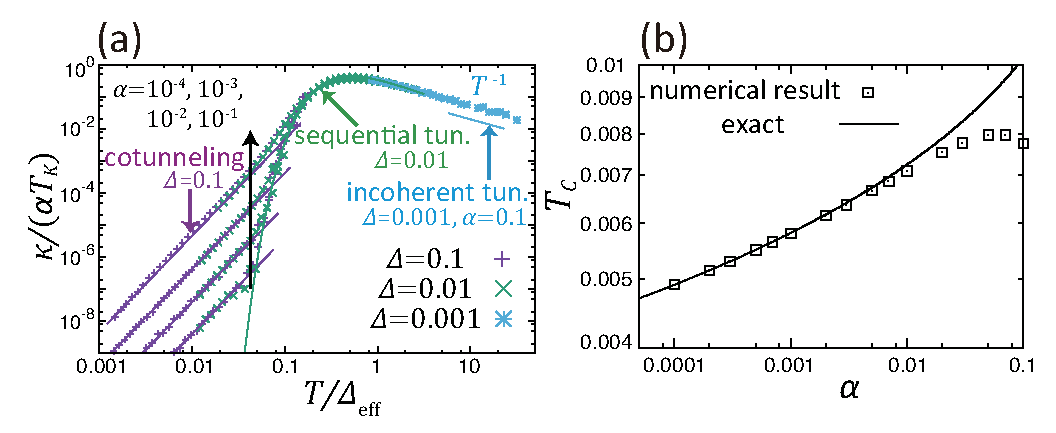
\includegraphics[width=165mm]{conductance_s1.eps}
 \caption{
	(a)オーミック散逸における熱コンダクタンスの温度依存性、(b)クロスオーバー温度$T_c$と結合定数$\alpha$の関係($\Delta=0.01$)。
		(a)では、グラフは両対数スケールとしており、データ点は量子モンテカルロ法による計算結果で、各データはボトムからトップまでそれぞれ$\alpha=10^{-4}(\rm{bottom}), 10^{-3},10^{-2},10^{-1}(\rm{top})$に対応している。ただし、$\Delta=0.001$については$\alpha=0.1$のみの計算結果である。紫色の実線が$\Delta=0.1$におけるcotunneling機構の式(\ref{cond_lowtemp})を$\alpha$で除した近似曲線、緑色の実線は$\Delta=0.01$におけるsequential tunneling機構の式(\ref{compare_ruokola2})を$\alpha$で除した近似曲線である。量子モンテカルロ計算においては、$5\times10^4$熱化ステップ、$25\times10^5$モンテカルロステップで計算を行った。(b)では、データ点は式(\ref{cond_lowtemp})と式(\ref{compare_ruokola2})の近似曲線の交点を求めることで計算したcotunnelingからsequential tunnelingへのクロスオーバー温度$T_c$であり、実線は解析的に求めた$T_c$と$\alpha$の関係を表す。
	}
	\label{fig:conductance_s1}
\end{figure}

より詳しく温度依存性を調べるために、ここではまず散逸強度$\alpha$が小さい場合を議論する。
図\ref{fig:conductance_s1}~(a)にオーミック散逸($\alpha = 10^{-4}, 10^{-3}, 10^{-2}, 10^{-1}$)における熱コンダクタンスの
温度依存性の計算結果を示す。ここでは逆温度$\beta$($=N$)は$\beta=64$から$\beta=8192$までとり、広い温度領域で
精度良く計算を行うために量子トンネル振幅を$\Delta/\omega_c=10^{-3},10^{-2},10^{-1}$とした。このグラフでは
熱コンダクタンス$\kappa$を、$\Delta_{\rm eff}/k_{\rm B}$だけでなく$\alpha$でも割っている。
これは、sequential tunneling機構による熱輸送が行われている時、計算データが同一曲線に乗るようにするためである。
図\ref{fig:conductance_s1}(a)のグラフから明らかなように、温度の上昇に伴い熱コンダクタンスがcotunneling機構による
温度依存性からsequential tunneling機構による温度依存性へとクロスオーバーしている様子がみてとれる。
また両者の機構の近似解と数値計算結果はよく一致していることがわかる。

次にcotunnelingからsequential tunnelingへのクロスオーバー温度$T_c$を見積もるため、$\Delta=0.1$において、sequential tunneling機構による
解析解(\ref{compare_ruokola2})(図\ref{fig:conductance_s1}(a)の緑色の曲線)と、$\alpha$の値を変化させた時のcotunneling機構による解析解(\ref{cond_lowtemp})(図\ref{fig:conductance_s1}(a)の紫色の曲線)の交点を数値的に決めた。
ただし、cotunneling機構の解析解(\ref{cond_lowtemp})中の帯磁率$\chi_m$は数値計算による結果を用いた。
その結果を図\ref{fig:conductance_s1}~(b)のデータ点に示す。クロスオーバー温度$T_c$より低温側がcotunneling領域、
高温側がsequential tunneling領域である。また、摂動論による近似計算では、解析解
(\ref{cond_lowtemp})の表式において$\chi_m$を$2/\Delta$とした結果が得られ、クロスオーバー温度$T_c$は
\begin{eqnarray}
T_c^5\sinh\left(\frac{\Delta}{T_c}\right)= \frac{\Delta^5}{4\alpha F(1)}
\end{eqnarray}
を数値的に解くことで得られる。ここで、$F(1)$は式(\ref{cond_lowtemp})の$F(s=1)$を意味する。
この結果を図\ref{fig:conductance_s1}~(b)の実線に示す。摂動論による結果は$\alpha=0.01$程度までは、
帯磁率を数値計算したものとよく一致しているが、$\alpha$がそれ以上大きくなるとずれてくることがわかる。

最後に$\alpha\geq1$での熱コンダクタンスを議論する。この領域では$T_K=0$となるため、
有限温度でcotunneling機構は発現しない。また、量子力学的な重ね合わせ状態は完全に破壊されてしまっているので、
sequential tunneling機構も働かず、すべての温度領域でincoherent tunnelingによる熱輸送が生じることがわかる。
図\ref{fig:ohmic_incoherent_tunneling}に$\alpha=1, 1.25, 1.5, 1.75, 2.0$のときの熱コンダクタンスの温度依存性を示す。
データ点はモンテカルロ計算の結果を表し、実線はincoherent tunnelingの解析解(\ref{ohmic_incoherent})を示す。ただし、式(\ref{ohmic_incoherent})をそのまま用いるとデータ点との
ずれが生じるため、$\omega_c$を$2\omega_c$と取り直している。この違いは、もとのスピン・ボゾン模型を
イジング模型にマップする際に生じるものであると考えられる。実際、この違いはただ単に$T_K$の大きさを少し
変えるだけの効果を持ち、図\ref{fig:ohmic_result}のようなスケーリング曲線(エネルギーを$T_K$で規格化したときに
得られる曲線)に直したときは違いが現れない。

\begin{figure}[tb]
 \centering
 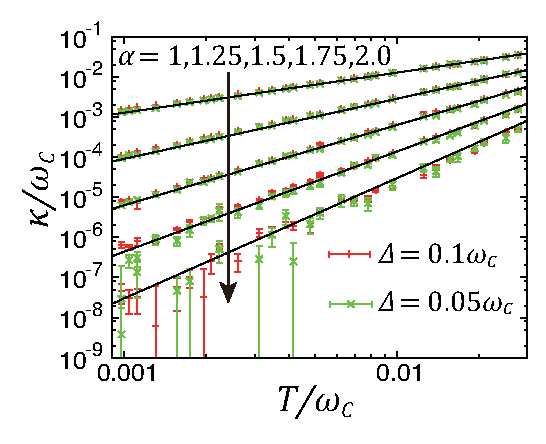
\includegraphics[width=80mm]{ohmic_incoherent_tunneling.eps}
 \caption{
	$\alpha\geq1$におけるオーミック散逸の熱コンダクタンスの温度依存性。各データはトップから	ボトムまでそれぞれ$\alpha=1.0(\rm top),1.25,1.5,1.75,2.0(\rm bottom)$に対応している。実線は	incoherent tunnelingの近似曲線(\ref{ohmic_incoherent})である。
   }
   \label{fig:ohmic_incoherent_tunneling}
\end{figure}

%==================================================
\subsubsection{Super ohmic case}

スーパーオーミック散逸($s>1$)は散逸の効果は弱く、常に式(\ref{super_ohmic_kurikomi})で与えられるような
有効相互作用$\Delta_{\rm eff}$を定義できる。ここでは$s=2.0$および$s=1.5$のスーパーオーミック散逸における
熱コンダクタンスの温度依存性を議論する。

\begin{figure}[tb]
	\centering
	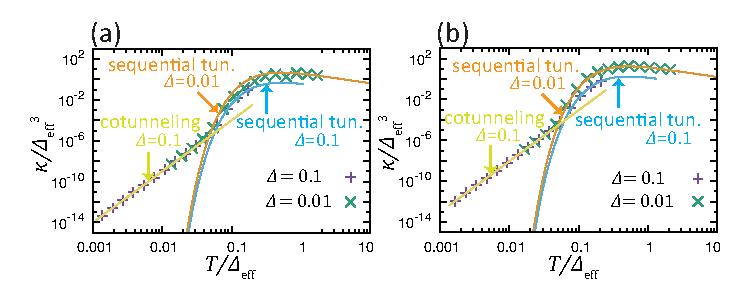
\includegraphics[height=5.7cm]{conductance_s2.0.eps}
	\caption{
	$s=2.0$のスーパーオーミック散逸における熱コンダクタンスの温度依存性: (a) $\alpha=0.1$、(b) $\alpha=0.3$。
	両対数スケールとしており、データ点は量子モンテカルロ法による計算結果、
	黄色の実線が$\Delta_{\mathrm{eff}}=0.1$におけるcotunneling機構の近似曲線(\ref{cond_lowtemp})、水色と橙色の実線はそれぞれ$\Delta_{\mathrm{eff}}=0.1,\ 0.01$におけるsequential tunneling機構の近似曲線(\ref{compare_ruokola2})である。
		量子モンテカルロ計算においては、$10^6$熱化ステップ、$5\times10^7$モンテカルロステップで計算を行った。
	}
	\label{fig:conductance_s2.0}
\end{figure}

まず、$s=2.0$のときの熱コンダクタンスの温度依存性を議論する。結合定数$\alpha=0.1$, $0.3$とした場合の結果を
図\ref{fig:conductance_s2.0}の(a)と(b)にそれぞれ示す。
ここで、$s$を変化させたときに次元を保つため、縦軸を$\Delta_{\mathrm{eff}}^{2s-1}$で割っている。
データ点はモンテカルロ計算の結果を表し、高温側の実線はsequential tunneling機構の式(\ref{compare_ruokola2})、低温側の実線は
cotunneling機構の式(\ref{cond_lowtemp})を表す。低温側ではcotunneling機構による熱輸送によってよく説明されるのに対し、
高温側ではsequential tunneling機構による熱輸送によってよく説明されることがわかる。
また同時に、式(\ref{shiba})の一般化斯波関係式がスーパーオーミック散逸の低温領域で確かに成り立つことも、
この計算によって示唆される。
$s=2.0$のスーパーオーミック散逸では量子力学的な重ね合わせ状態を破壊することはないため、
incoherent tunneling機構の熱輸送は生じない。これらの特徴は$s>2$のスーパーオーミック散逸でも同様に
成り立つと期待される。

\begin{figure}[tb]
	\centering
	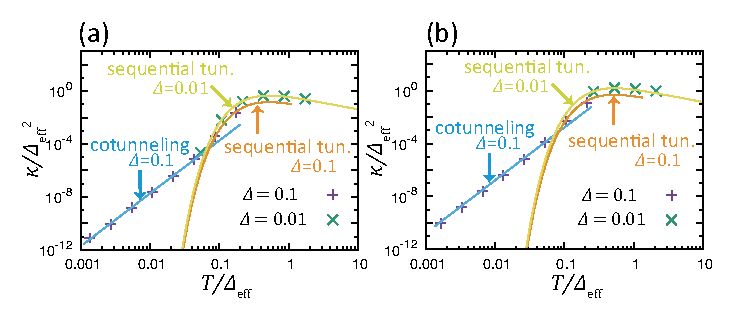
\includegraphics[height=6.0cm]{conductance_s1.5.eps}
	\caption{
	$s=1.5$のスーパーオーミック散逸における熱コンダクタンスの温度依存性: (a) $\alpha=0.1$、(b) $\alpha=0.3$。
	両対数スケールとしており、データ点は量子モンテカルロ法による計算結果、
	水色の実線が$\Delta=0.1$におけるcotunneling機構の近似曲線(\ref{cond_lowtemp})、橙色と黄色の実線はそれぞれ$\Delta=0.1,\ 0.01$におけるsequential tunneling機構の近似曲線(\ref{compare_ruokola2})である。量子モンテカルロ計算においては、$10^6$熱化ステップ、$5\times10^7$モンテカルロステップで計算を行った。
	}
	\label{fig:conductance_s1.5}
\end{figure}

一方、$1<s<2$のスーパーオーミック散逸では、高温で重ね合わせ状態が破壊される場合がある。
それを具体的に見るために、$s=1.5$のスーパーオーミック散逸における熱コンダクタンスの温度依存性を議論する。
まず、熱浴との結合強度を比較的小さな値である$\alpha=0.1$, $0.3$とした場合の結果を、
図\ref{fig:conductance_s1.5}の(a)および(b)に示す。
データ点はモンテカルロ計算の結果を表し、高温側の実線はsequential tunneling機構の式(\ref{compare_ruokola2})、低温側の実線は
cotunneling機構の式(\ref{cond_lowtemp})を表す。
$s=2$の場合と同様に、低温側ではcotunneling機構による熱輸送が、
高温側ではsequential tunneling機構による熱輸送が実現されている。

\begin{figure}[tb]
	\centering
	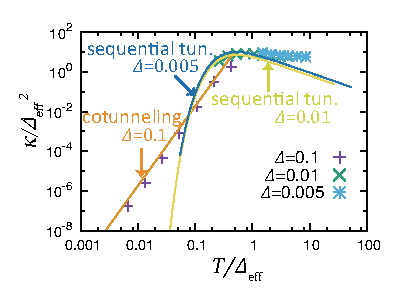
\includegraphics[height=6cm]{conductance_s1.5_alpha1.0.eps}
	\caption{
	$s=1.5,\alpha=1.0$のスーパーオーミック散逸における熱コンダクタンスの温度依存性。
	両対数スケールとしており、データ点は量子モンテカルロ法による計算結果、
	橙色の実線が$\Delta=0.1$におけるcotunneling機構の近似曲線(\ref{cond_lowtemp})、黄色と青色の実線はそれぞれ$\Delta=0.01,\ 0.005$におけるsequential tunneling機構の近似曲線(\ref{compare_ruokola2})である。
	量子モンテカルロ計算においては、$10^6$熱化ステップ、$5\times10^7$モンテカルロステップで計算を行った。
	}
	\label{fig:conductance_s1.5_alpha1.0}
\end{figure}

さらに熱浴との結合強度を$\alpha=1.0$とした結果を図\ref{fig:conductance_s1.5_alpha1.0}に示す。
この場合は、低温ではcotunnelingの近似解とよく合っているが、$T/\Delta_{\rm eff}$が$1$よりも大きくなるにつれて、
sequential tunnelingの表式からデータ点が乖離していく様子がわかる。これは温度ゆらぎによって
incoherent tunnelingが起こっているからと予想される。しかし、$1<s\leq2$ではフェルミの黄金律から
求まるトンネル確率$\Gamma$の式(\ref{Gamma})の指数部分$Q(t)$に特異点が現れ\cite{Weiss99}、$\Gamma$を容易に
導出することはできないため、本研究ではこの領域の熱コンダクタンスの近似解は導出しなかった。
ただし、別の角度からこの予想の妥当性を確かめることは可能である。
量子モンテカルロ法で計算した応答スペクトル関数$S(\omega)$(図\ref{fig:spect_delta0.01_alpha1.0})を見ると、
$N=512$ではデルタ関数で近似できるような$\omega=\pm \Delta_{\rm eff}$近傍に鋭い2つのピークを持つ関数になっているが、
$N$の減少に伴い徐々にピークが鈍くなり$N=64$ではLorentz型の関数となっている。
これは、第3章の議論を踏まえると、熱輸送機構がsequential tunnelingからincoherent tunnelingへとクロスオーバーしていることを意味する。

\begin{figure}[tb]
	\centering
	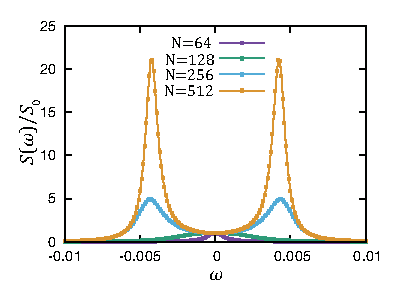
\includegraphics[height=6cm]{spect_delta0.01_alpha1.0.eps}
	\caption{
	$s=1.5,\alpha=1.0,\Delta=0.01$における応答スペクトル関数。
	縦軸は応答スペクトル関数$S(\omega)$を$\omega=0$におけるスペクトル関数の値$S_0$で割っている。温度の上昇($N$の減少)に伴いデルタ関数型のダブルピークからLorentz型のシングルピーク関数へのクロスオーバーが起こる。
	}
	\label{fig:spect_delta0.01_alpha1.0}
\end{figure}

%==================================================
\subsubsection{Sub ohmic case}

\begin{figure}[tb]
	\centering
	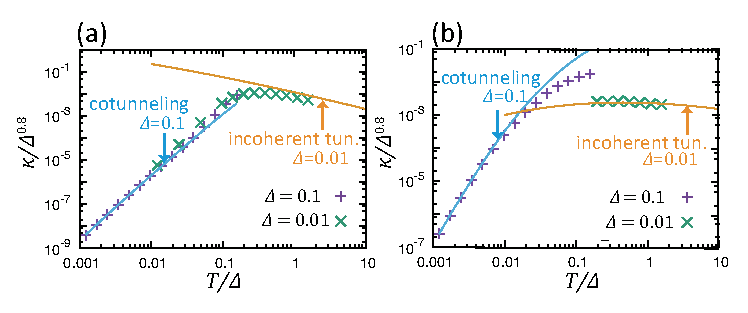
\includegraphics[height=6.0cm]{conductance_s0.9.eps}
	\caption{
	(a)$s=0.9$のサブオーミック散逸における熱コンダクタンスの温度依存性:(a)$\alpha=0.1$、(b)$\alpha=0.3$。
	両対数スケールとしており、データ点は量子モンテカルロ法による計算結果、
	水色の実線が$\Delta=0.1$におけるcotunneling機構の近似曲線(\ref{cond_lowtemp})、橙色の実線は$\Delta=0.01$におけるincoherent tunneling機構の近似曲線(\ref{sub_ohmic_hightemp})である。
	量子モンテカルロ計算においては、$10^6$熱化ステップ、$5\times10^7$モンテカルロステップで計算を行った。
	}
	\label{fig:conductance_s0.9}
\end{figure}

次にサブオーミック散逸における熱輸送を議論する。一般にサブオーミック散逸では$s$が小さくなるとイジング模型の
長距離相互作用が大きくなるため、Wolff法で形成されるクラスターサイズも非常に大きくなり、
結果として低温領域でモンテカルロ法の状態更新に膨大な時間を費やす。
そこで、$s$の値として極端に小さくない値$s=0.9$をまず調べる。
熱浴との結合強度を$\alpha=0.1$および0.3とした場合の結果を図\ref{fig:conductance_s0.9}に示す。
データ点はモンテカルロ計算の結果を表し、高温側の実線はincoherent tunneling機構の式(\ref{sub_ohmic_hightemp})、低温側の実線は
cotunneling機構の式(\ref{cond_lowtemp})を表す。

\begin{figure}[tb]
	\centering
	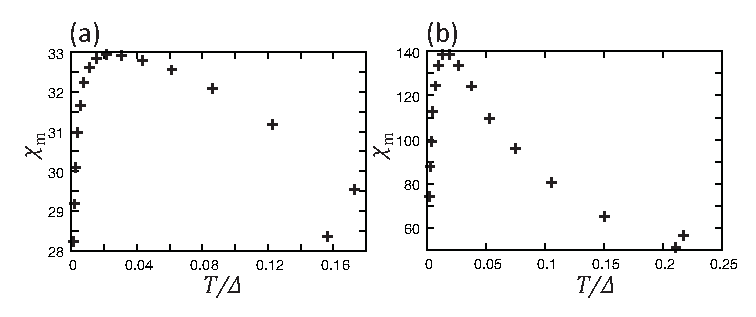
\includegraphics[height=6.0cm]{suceptibility_s0.9_delta0.1_alpha0.1-0.3.eps}
	\caption{
		$s=0.9,\Delta=0.1$おける帯磁率の温度依存性: (a)$\alpha=0.1$、(b)$\alpha=0.3$ 。
	}
	\label{fig:suceptibility_s0.9_delta0.1_alpha0.1-0.3}
\end{figure}

まず、低温の熱輸送はcotunnelingによって生じることが図\ref{fig:conductance_s0.9}からみてとれる。
ただし、cotunneling機構の式(\ref{cond_lowtemp})を用いるにあたっては、
数値計算で求めた帯磁率$\chi_m$(図\ref{fig:suceptibility_s0.9_delta0.1_alpha0.1-0.3})を利用した。
図\ref{fig:suceptibility_s0.9_delta0.1_alpha0.1-0.3}に示されるように、帯磁率$\chi_m$は低温で特異的な温度依存性を
示しており、図\ref{fig:conductance_s0.9}の低温でのデータ点を合わせるためには、この温度依存性を考慮する必要がある。
なお、図\ref{fig:suceptibility_s0.9_delta0.1_alpha0.1-0.3}に示される低温における帯磁率$\chi_m$の特異な振る舞いは、
サブオーミックで生じる量子相転移と何らかの関係があると期待される。
低温領域では、オーミックやスーパーオーミック散逸で現れるcotunnelingの温度依存性の振る舞い$T^{2s+1}$と比較すると、
低温での$\chi_m$の温度依存性によって$\kappa$が僅かに抑制されているが、ほぼ$2s+1$のべきに近い振る舞いが得られていることが
わかる。よって概ね、cotunnelingの$T^{2s+1}$に比例する温度依存性が低温で実現されていると言える。

一方、図\ref{fig:conductance_s0.9}より、高温の熱輸送は式(\ref{sub_ohmic_hightemp})のincoherent tunnelingによる熱輸送が生じていることが
わかる。サブオーミック散逸では散逸の影響が強いため、sequential tunnelingによる熱輸送は起こらないと考えられる。

数値計算上の議論として、先述の通りサブオーミック散逸では長距離相互作用がスーパーオーミック散逸のときと比べて大きいため、
低温領域で計算時間が非常に長くなる。これは量子モンテカルロ法の限界であり、本研究でも図\ref{fig:conductance_s0.9}(b)の計算では、
incoherent tunneling領域で$N=512$が計算可能な上限であった。これより低温を見るには量子モンテカルロ法のアルゴリズムの
変更などの工夫が必要である。

%==================================================
\subsection{Phase transition in sub ohmic regime}
\label{sec:phasetransition}

局在転移とは、温度ゼロ($\beta = N \rightarrow \infty$)において量子力学的な摩擦$\alpha$が臨界摩擦$\alpha_c$を超えると、
トンネル効果が全く起こらなくなり($\Gamma\rightarrow0$)波動関数が局在化する現象である。
これを調べるために、次のように定義されるBinderパラメーターを導入する。
\begin{eqnarray}
	B\equiv\frac{1}{2}\left(3-\frac{\average{\sigma_z}^4}{\average{\sigma_z^2}^2}\right)
\end{eqnarray}
Binderパラメーターは相転移の臨界係数を決めるのに有効な物理量として知られている。 
\begin{figure}[tb]
	\centering
	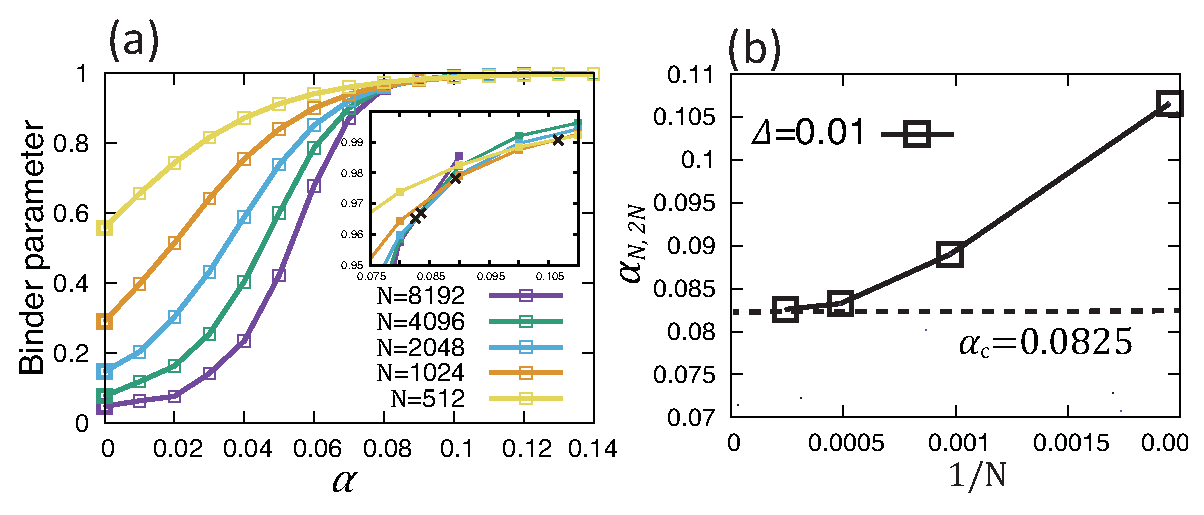
\includegraphics[height=6.0cm]{binder_parameter.eps}
	\caption{
	(a)$s=0.6,\ \Delta=0.01$におけるBinderパラメーターの$\alpha$依存性、(b)Binderパラメーターの交点。 (a)の埋め込み図中の×印は$N$と$2N$におけるBinderパラメーターの交点を表す。(b)中の点線はフィッティングで得た零点近傍の漸近線である。
	}
	\label{fig:binder_parameter}
\end{figure}

$s=0.6$, $\Delta=0.01$のサブオーミック散逸において、Binderパラメーターの$\alpha$依存性を調べた結果が
図\ref{fig:binder_parameter}(a)である。このパラメーターに対して、Binderパラメーターは$\alpha=0.09$付近で交点を持つ。
拡大図を図\ref{fig:binder_parameter}(a)中の挿入図に示す。ここで、局在転移は$T\rightarrow0(N\rightarrow\infty)$で起こるので、
$N$と$2N$におけるBinderパラメーターの交点を$\alpha_{N,2N}$とすると、
$\alpha_{N,2N}$は$N$の増加に伴って臨界摩擦$\alpha_c$に収束するはずである。
データから$\alpha_{N,2N}$を求め、その$N$依存性を調べたグラフが図\ref{fig:binder_parameter}(b)である。
$N$を大きくするに従い、$\alpha_{N,2N}$がある値に収束する様子がみてとれる。
$1/N$の二次関数によって$\alpha_{N,2N}$をフィットし、外挿によって$N\rightarrow\infty$での$\alpha_c$を計算すると、
図\ref{fig:binder_parameter}(b)の場合は$\alpha_c=0.0825$と求まる。

\begin{figure}[tb]
	\centering
	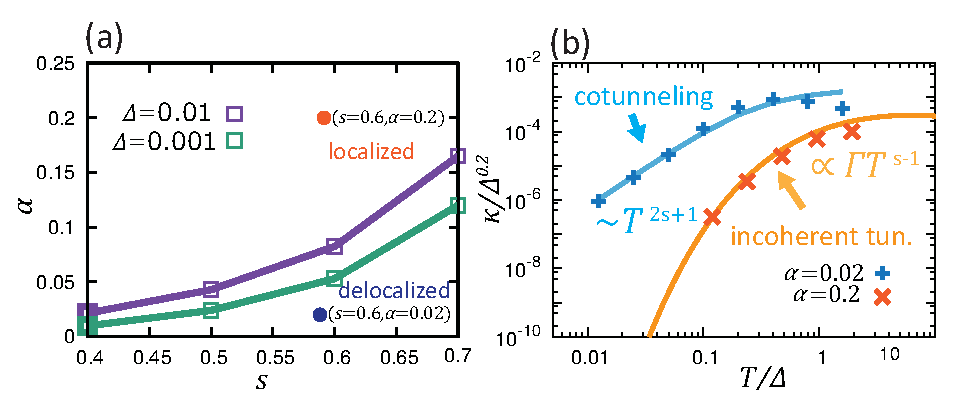
\includegraphics[height=6.0cm]{localization_phasediagram.eps}
	\caption{
	(a)$T=0$における局在転移の相図、 (b)$\Delta=0.01$での局在相$(s=0.6,\alpha=0.2)$・非局在相$(s=0.6,\alpha=0.02)$における熱コンダクタンスの温度依存性。
	水色の実線が$\Delta=0.01,\alpha=0.02$におけるcotunneling機構の近似曲線(\ref{cond_lowtemp})、橙色の実線は$\Delta=0.01,\alpha=0.2$におけるincoherent tunneling機構の近似曲線(\ref{sub_ohmic_hightemp})である。
	}
	\label{fig:localization_phasediagram}
\end{figure}

この手続きを$s<1$を満たす各$s$に対して行った結果、 $\alpha$と$s$についての局在転移の相図が得られる(図\ref{fig:localization_phasediagram}(a))。
この結果は先行研究の数値くりこみ群による結果\cite{Vojta05}と定量的におおよそ一致している。ここでは相図の中で、
$\Delta=0.01$に対して局在相を代表する点$(s,\alpha) = (0.6,0.2)$および非局在相を代表する点$(s,\alpha) = (0.6,0.02)$の2点で、
熱コンダクタンスの温度依存性を示したのが図\ref{fig:localization_phasediagram}(b)である。
局在相のパラメーター$(s,\alpha) = (0.6,0.2)$ではすべての温度領域でincoherent tunnelingによる熱輸送でよく記述されるのに対し、
非局在相のパラメーター$(s,\alpha) = (0.6,0.02)$では低温でcotunnelingによる熱輸送が生じていることがわかる。
ただし、非局在相のパラメーター$(s,\alpha) = (0.6,0.02)$では、高温でincoherent tunnelingによる熱輸送へとクロスオーバーすると期待されるが、
数値計算の精度の問題により、そこまでの温度領域の計算ができなかった。
このように、量子相転移によって波動関数が局在すると、cotunneling領域がなくなり、
熱コンダクタンスの温度依存性が大きく変わることがわかる。最後に、温度$T$と結合強度$\alpha$に関する相図の模式図を
図\ref{fig:sub_ohmic_phasediagram}にまとめる。

\begin{figure}[tb]
	\centering
	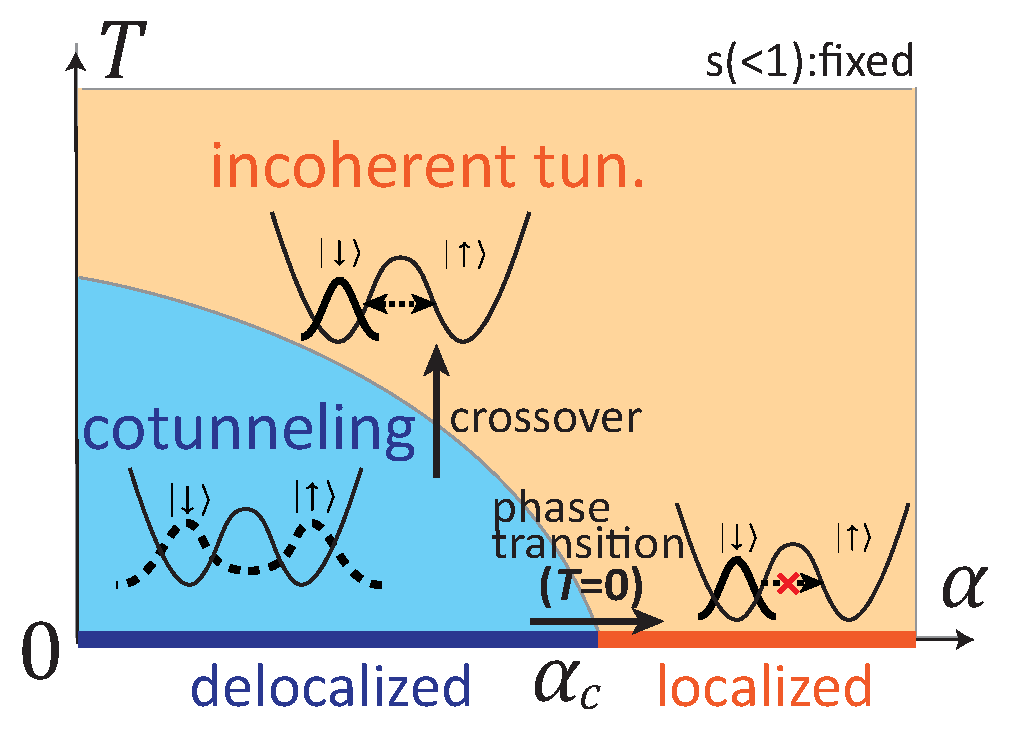
\includegraphics[height=7.0cm]{sub_ohmic_phasediagram.eps}
	\caption{
	サブオーミック散逸における熱輸送機構の相図。
	}
	\label{fig:sub_ohmic_phasediagram}
\end{figure}

\section{Summary}

\begin{thebibliography}{99}

\bibitem{GoldhaberGordon98} 
D. Goldhaber-Gordon et al., Nature {\bf 391}, 156 (1998).

\bibitem{vanderWiel00}
W. van der Wiel et al., Science {\bf 289}, 2105 (2000).

\bibitem{Hewson97}
A. C. Hewson, {\em The Kondo Problem to Heavy Fermions}, 
(Cambridge University Press, Cambridge, 1997).

\bibitem{}

\bibitem{Leggett87} 
A. J. Leggett, S. Chakravarty, A. T. Dorsey, M. P. A. Fisher, A. Garg and W. Zwerger, Rev. Mod. Phys. {\bf 59}, 1(1987).

\bibitem{Volker98} 
K. V\"olker, Phys. Rev B {\bf 58}, 1862 (1998).

\bibitem{Cardy81} J. Cardy, J. Phys. A \textbf{14}, 1407 (1981).

\bibitem{MetropolisMethod} D. P. Landau and K. Binder, {\it A Guide to Monte Carlo Simulations in Statistical Physics} 2nd edition, (Cambridge University Press, UK, 2005).

\bibitem{Guinea85} 
F. Guinea, V. Hakim and A. Muramatsu, Phys. Rev. B {\bf 32}, 4410 (1985);
F. Guinea, Phys. Rev. B {\bf 32}, 4486 (1985).

\bibitem{Weiss99} 
U. Weiss, {\em Quantum Dissipative Systems} 4th Edition, (World Scientific, Singapore, 1999).

\bibitem{Meir92} 
Y. Meir and N. S. Wingreen, Phys. Rev. Lett. {\bf 68}, 2512 (1992).

\bibitem{Saito13}
% Kondo Signature in Heat Transfer via a Local Two-State System
K. Saito and T. Kato, Phys. Rev. Lett. {\bf 111}, 214301 (2013).

\bibitem{Saito08}
K. Saito, Europhys Lett. \textbf{83}, 50006 (2008) 


\bibitem{Wolff89} 
U. Wolff, Phys. Rev. Lett. {\bf 62}, 361 (1989).

\bibitem{Luijten95}
E. Luijten and H. W. Bl\"ote, Int. J. Mod. Phys. C \textbf {6}, 359 (1995).

\bibitem{Shiba75}
% Shiba relation
H. Shiba, Prog. Theor. Phys. {\bf 54}, 967 (1975).

\bibitem{Grabert85} 
H. Grabert and U. Weiss, Phys. Rev. Lett. {\bf 54}, 1605 (1985).

\bibitem{Fisher85} 
M. P. A. Fisher and A. T. Dorsey, Phys. Rev. Lett. {\bf 54}, 1609 (1985).

\bibitem{Ojanen08} 
T. Ojanen and A. -P. Jauho, Phys. Rev. Lett. {\bf 100}, 155902 (2008).

\bibitem{Segal13}
% Qubit-mediated energy transfer between thermal reservoirs: Beyond the Markovian master equation
D. Segal, Phys. Rev. B {\bf 87}, 195436 (2013).

%% Non-equilibrium heat transport
\bibitem{Segal14} 
% Heat transfer in the spin-boson model: A comparative study in the incoherent tunneling regime
D. Segal, Phys. Rev. E {\bf 90}, 012148 (2014).

\bibitem{Wang15}
%Nonequilibrium Energy Transfer at Nanoscale: A Uni ed Theory from Weak to Strong Coupling
C. Wang, J. Ren, and J. Cao, Scientific Reports {\bf 5}, 11787 (2015).

\bibitem{Ren10} 
J. Ren, P. H\"{a}nggi and B. Li, Phys. Rev. Lett. {\bf 104}, 170601 (2010).

\bibitem{Chen13}
 T. Chen, X.B. Wang and J. Ren, Phys. Rev. B {\bf 87}, 144303 (2013).

\end{thebibliography}
\end{document}

